\subsection{Key Neutronics Parameters Verification}
\begin{frame}
    \frametitle{AHTR Temperature Model Setup}
    For successful AHTR Moltres simulation, I must establish suitable spatial and
    energy homogenization that preserves accuracy while maintaining an acceptable
    runtime
    \begin{block}{Steps to produce Moltres AHTR Temperature Model}
        \begin{itemize}
          \item OpenMC neutronics model produces group constants for the Moltres model
          \item Mesh generation
          \item Moltres temperature model accepts group constants and mesh
        \end{itemize}
    \end{block}
    \begin{block}{Energy Homogenization}
        \begin{table}[]
            \centering
            \begin{minipage}[c]{0.6\textwidth}
                \centering
                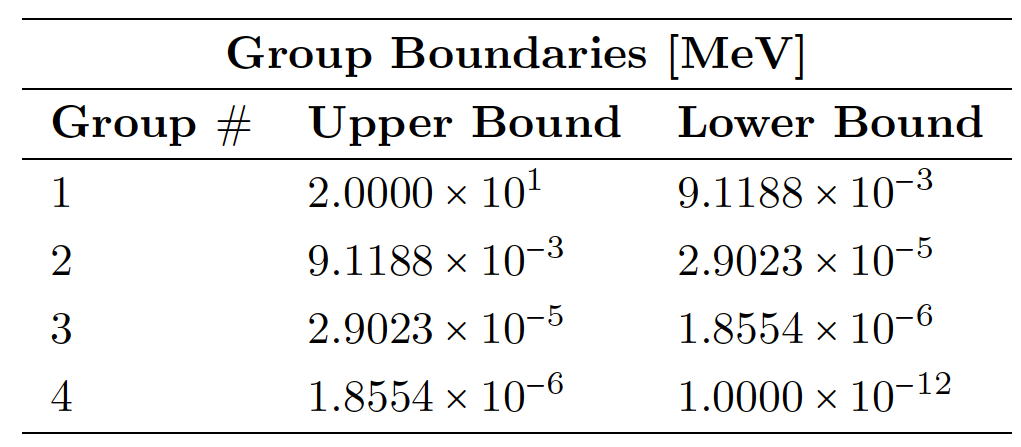
\includegraphics[width=0.8\linewidth]{figures/ahtr-energy-discr.png}
            \end{minipage}\hfill
            \begin{minipage}[c]{0.4\textwidth}
            \caption{4-group energy structures for AHTR geometry 
            derived by \cite{gentry_development_2016}.}
        \end{minipage}
        \end{table}
    \end{block}
\end{frame}

\begin{frame}
    \frametitle{AHTR Temperature Model Spatial Homogenization}
        \textbf{Fuel assembly 61 cell discretization}: inter-assembly FLiBe, 
        Y-shaped graphite structure, control rod slot FLiBe, graphite spacers, 
        each diamond shape section's inter-plank FLiBe (3), each graphite plank (18), 
        and each fuel stripe (36)
    \begin{figure}[]
            \centering
            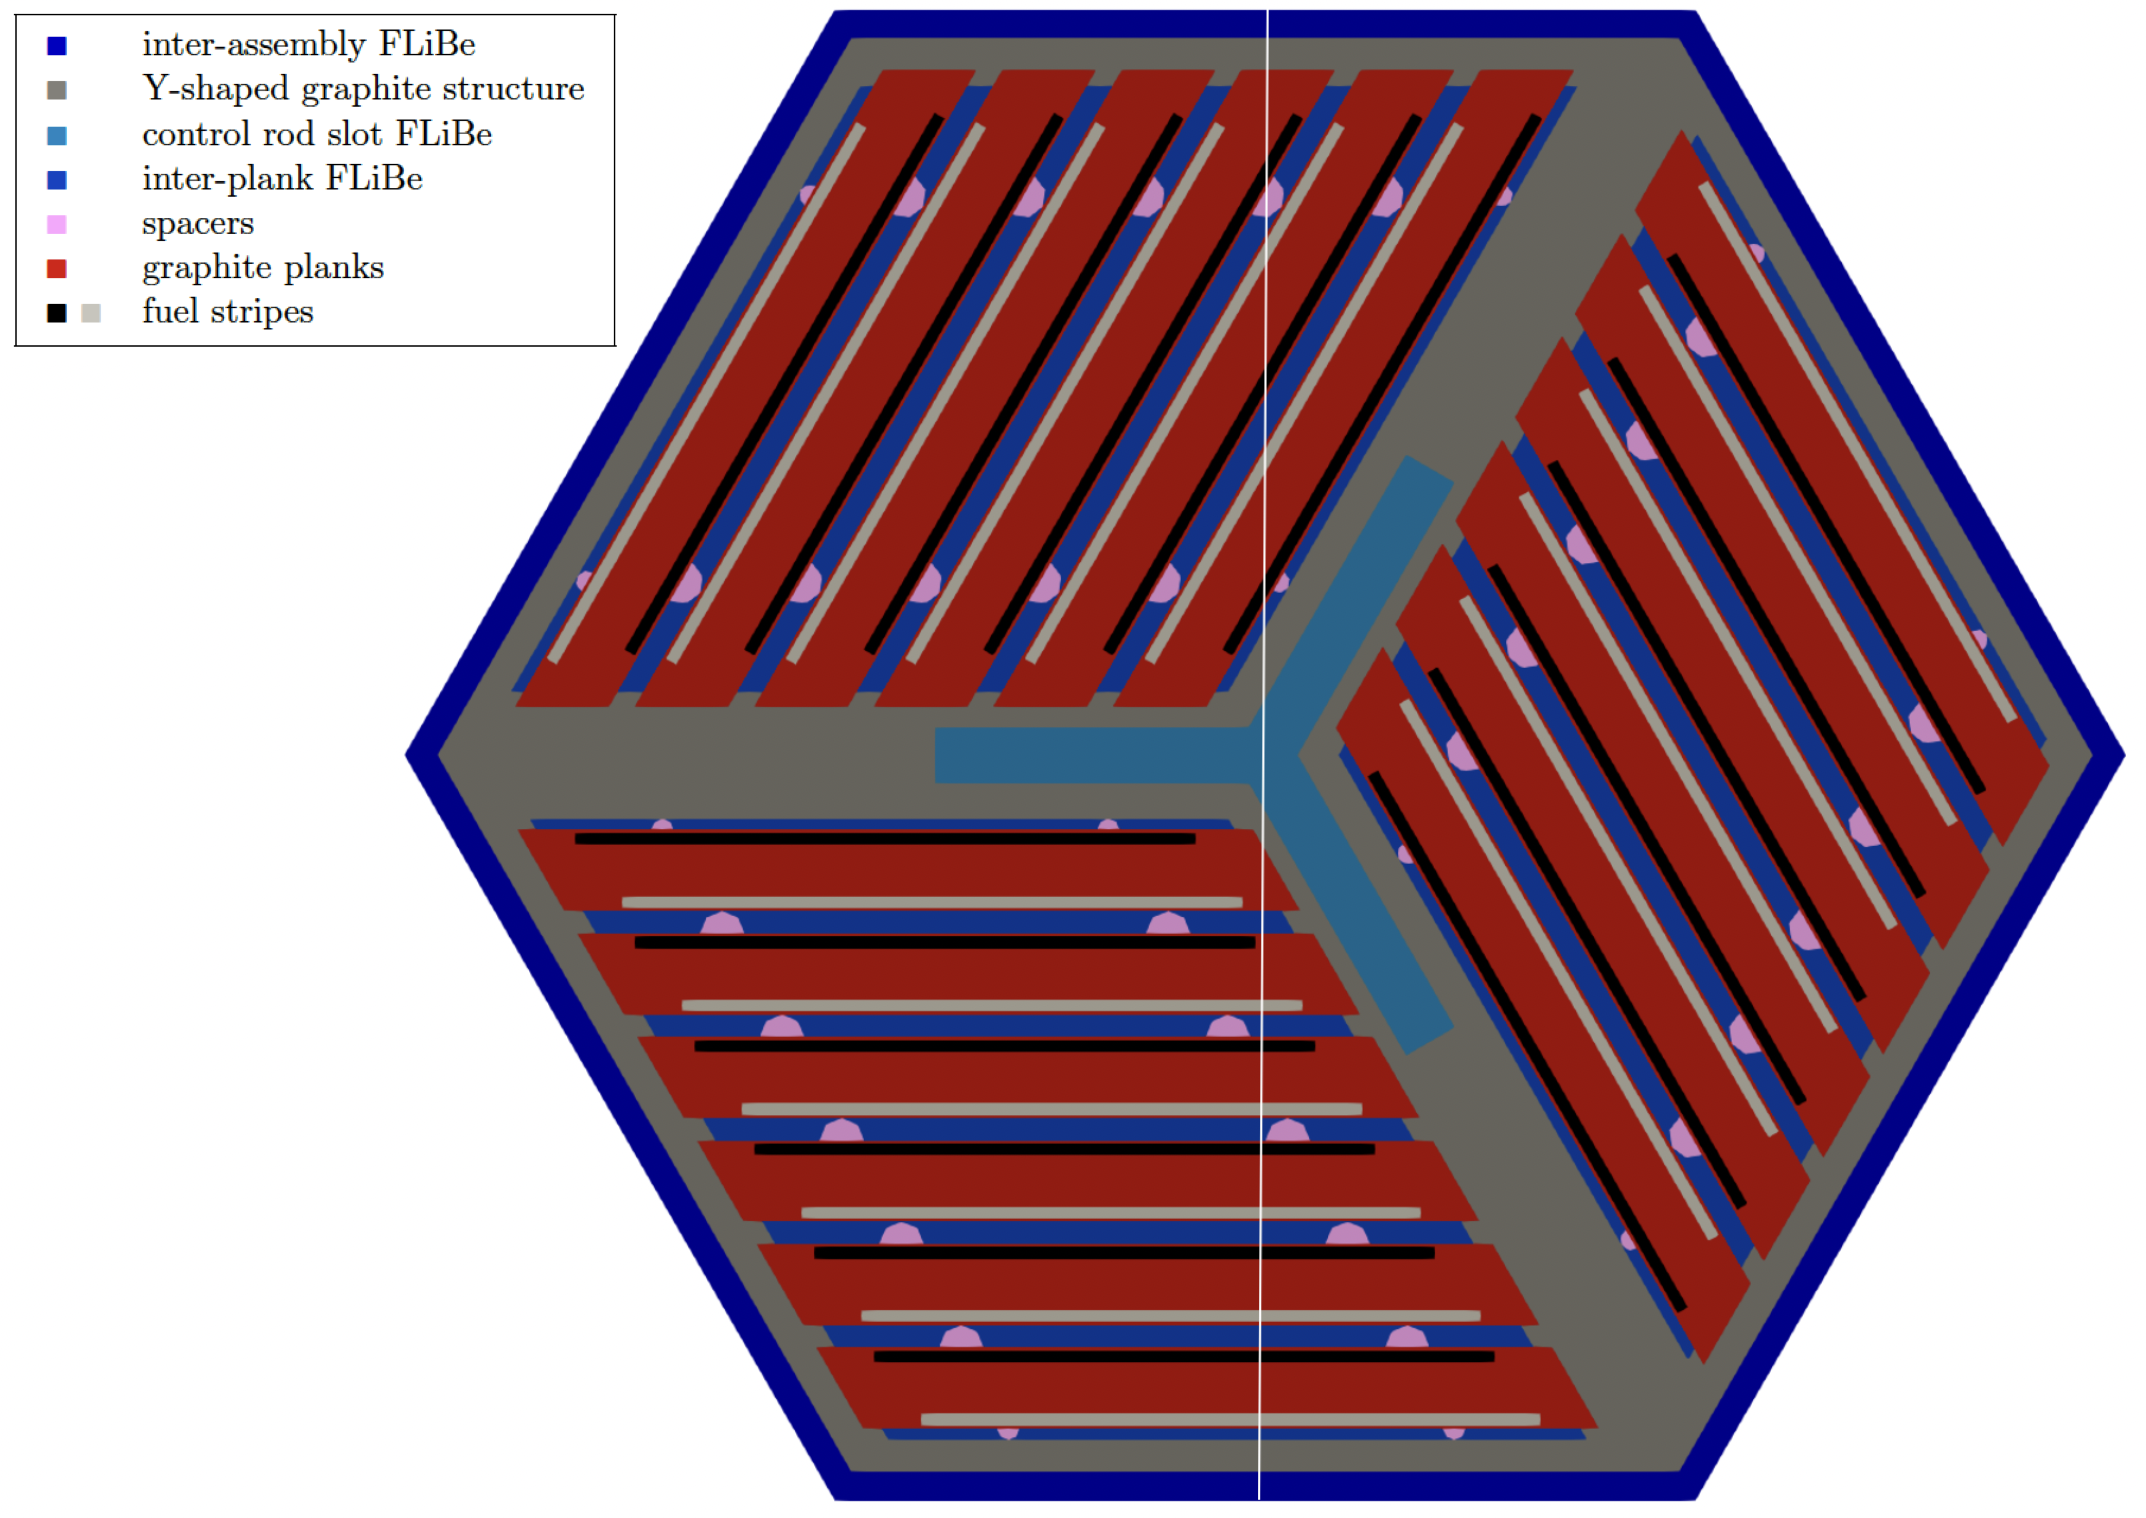
\includegraphics[width=0.65\linewidth]{figures/assembly_mg_pres.png}
        \caption{AHTR Assembly Spatial Homogenization for Group Constant Generation.}
    \end{figure}
\end{frame}

\begin{frame}
    \frametitle{AHTR Temp Model Key Neutronics Parameter Verification}
    I \textbf{verify acceptable spatial homogenization and energy discretization} by 
    comparing key neutronics parameters (KNPs) between: 
    \begin{itemize} 
        \item OpenMC simulation with continuous energy and TRISO-level spatial fidelity
        \item Moltres simulation with 4-group energy and spatial homogenization
    \end{itemize}
    \textbf{KNPs}: $k_{eff}$, reactivity coefficients, flux distribution, and neutron spectrum. 
        \begin{table}
            \caption{ $k_{eff}$ comparison.}
            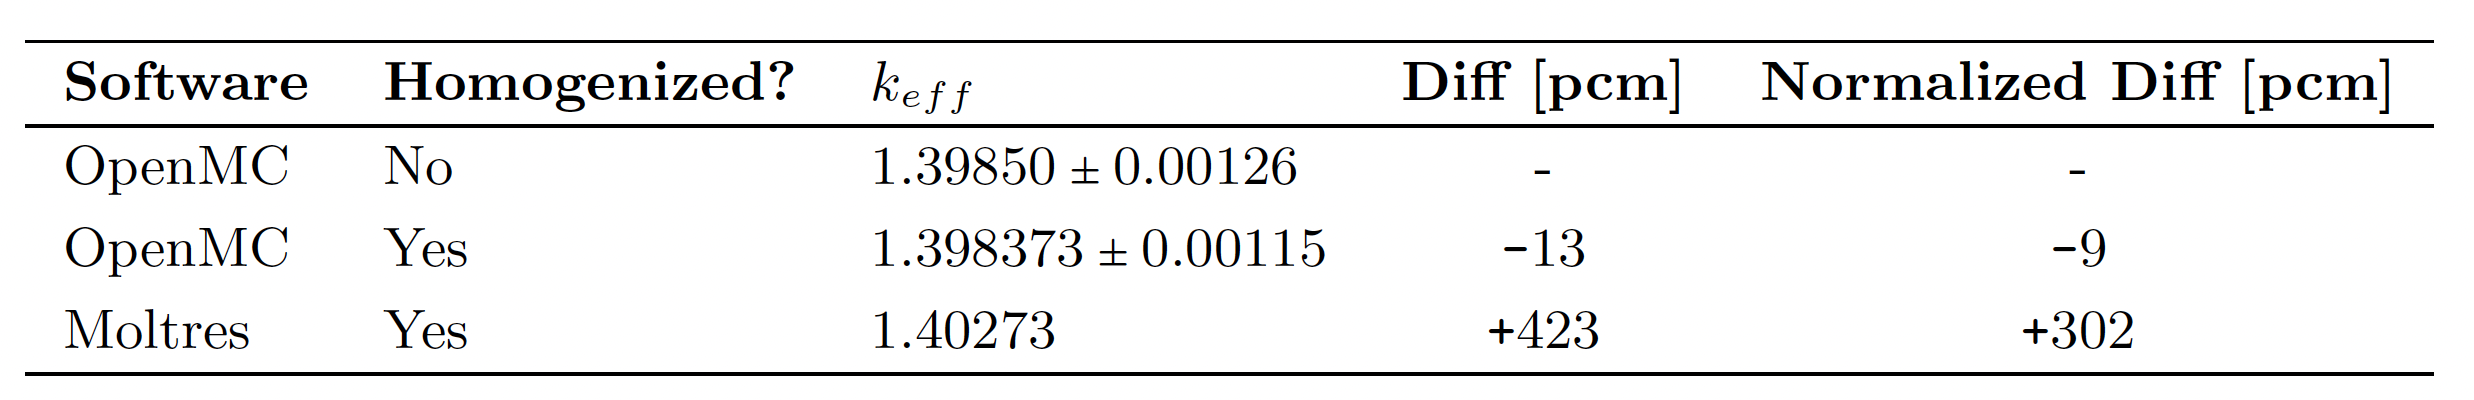
\includegraphics[width=0.85\linewidth]{figures/benchmark-keff.png}
        \end{table}
        \begin{table}
            \caption{Reactivity coefficients comparison.}
            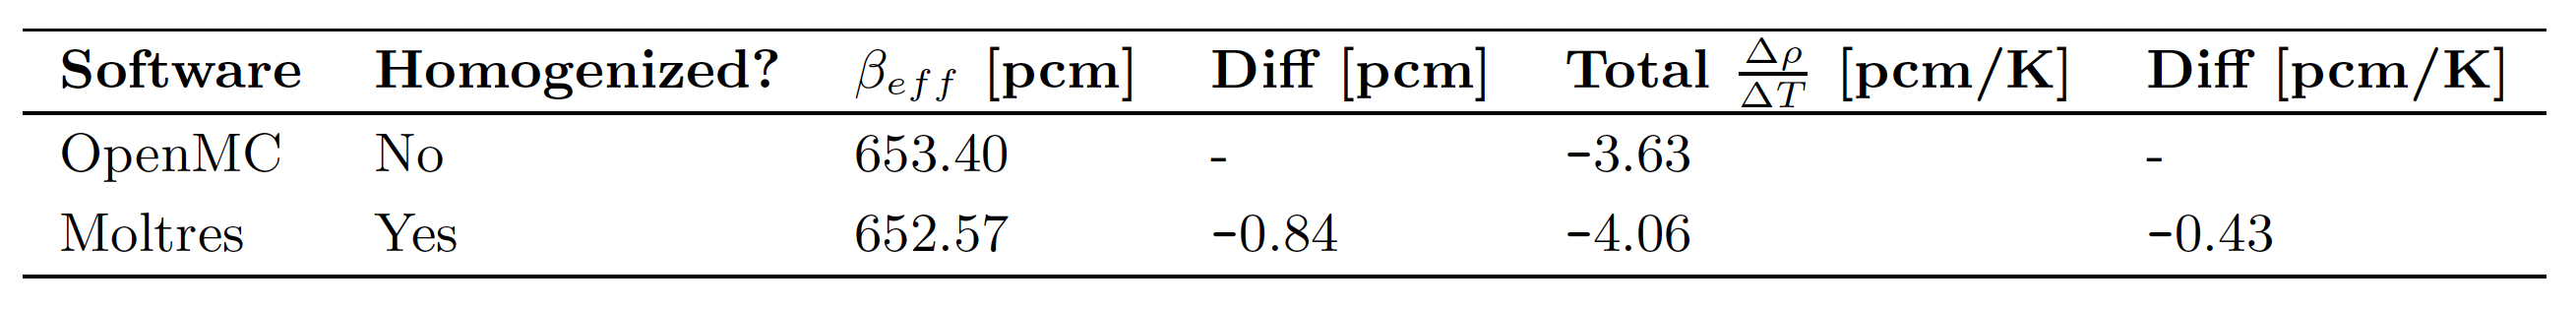
\includegraphics[width=0.85\linewidth]{figures/benchmark-coeff.png}
        \end{table}
\end{frame}

\begin{frame}
    \frametitle{AHTR Temp Model Flux Verification}
    \begin{figure}[]
        \centering
        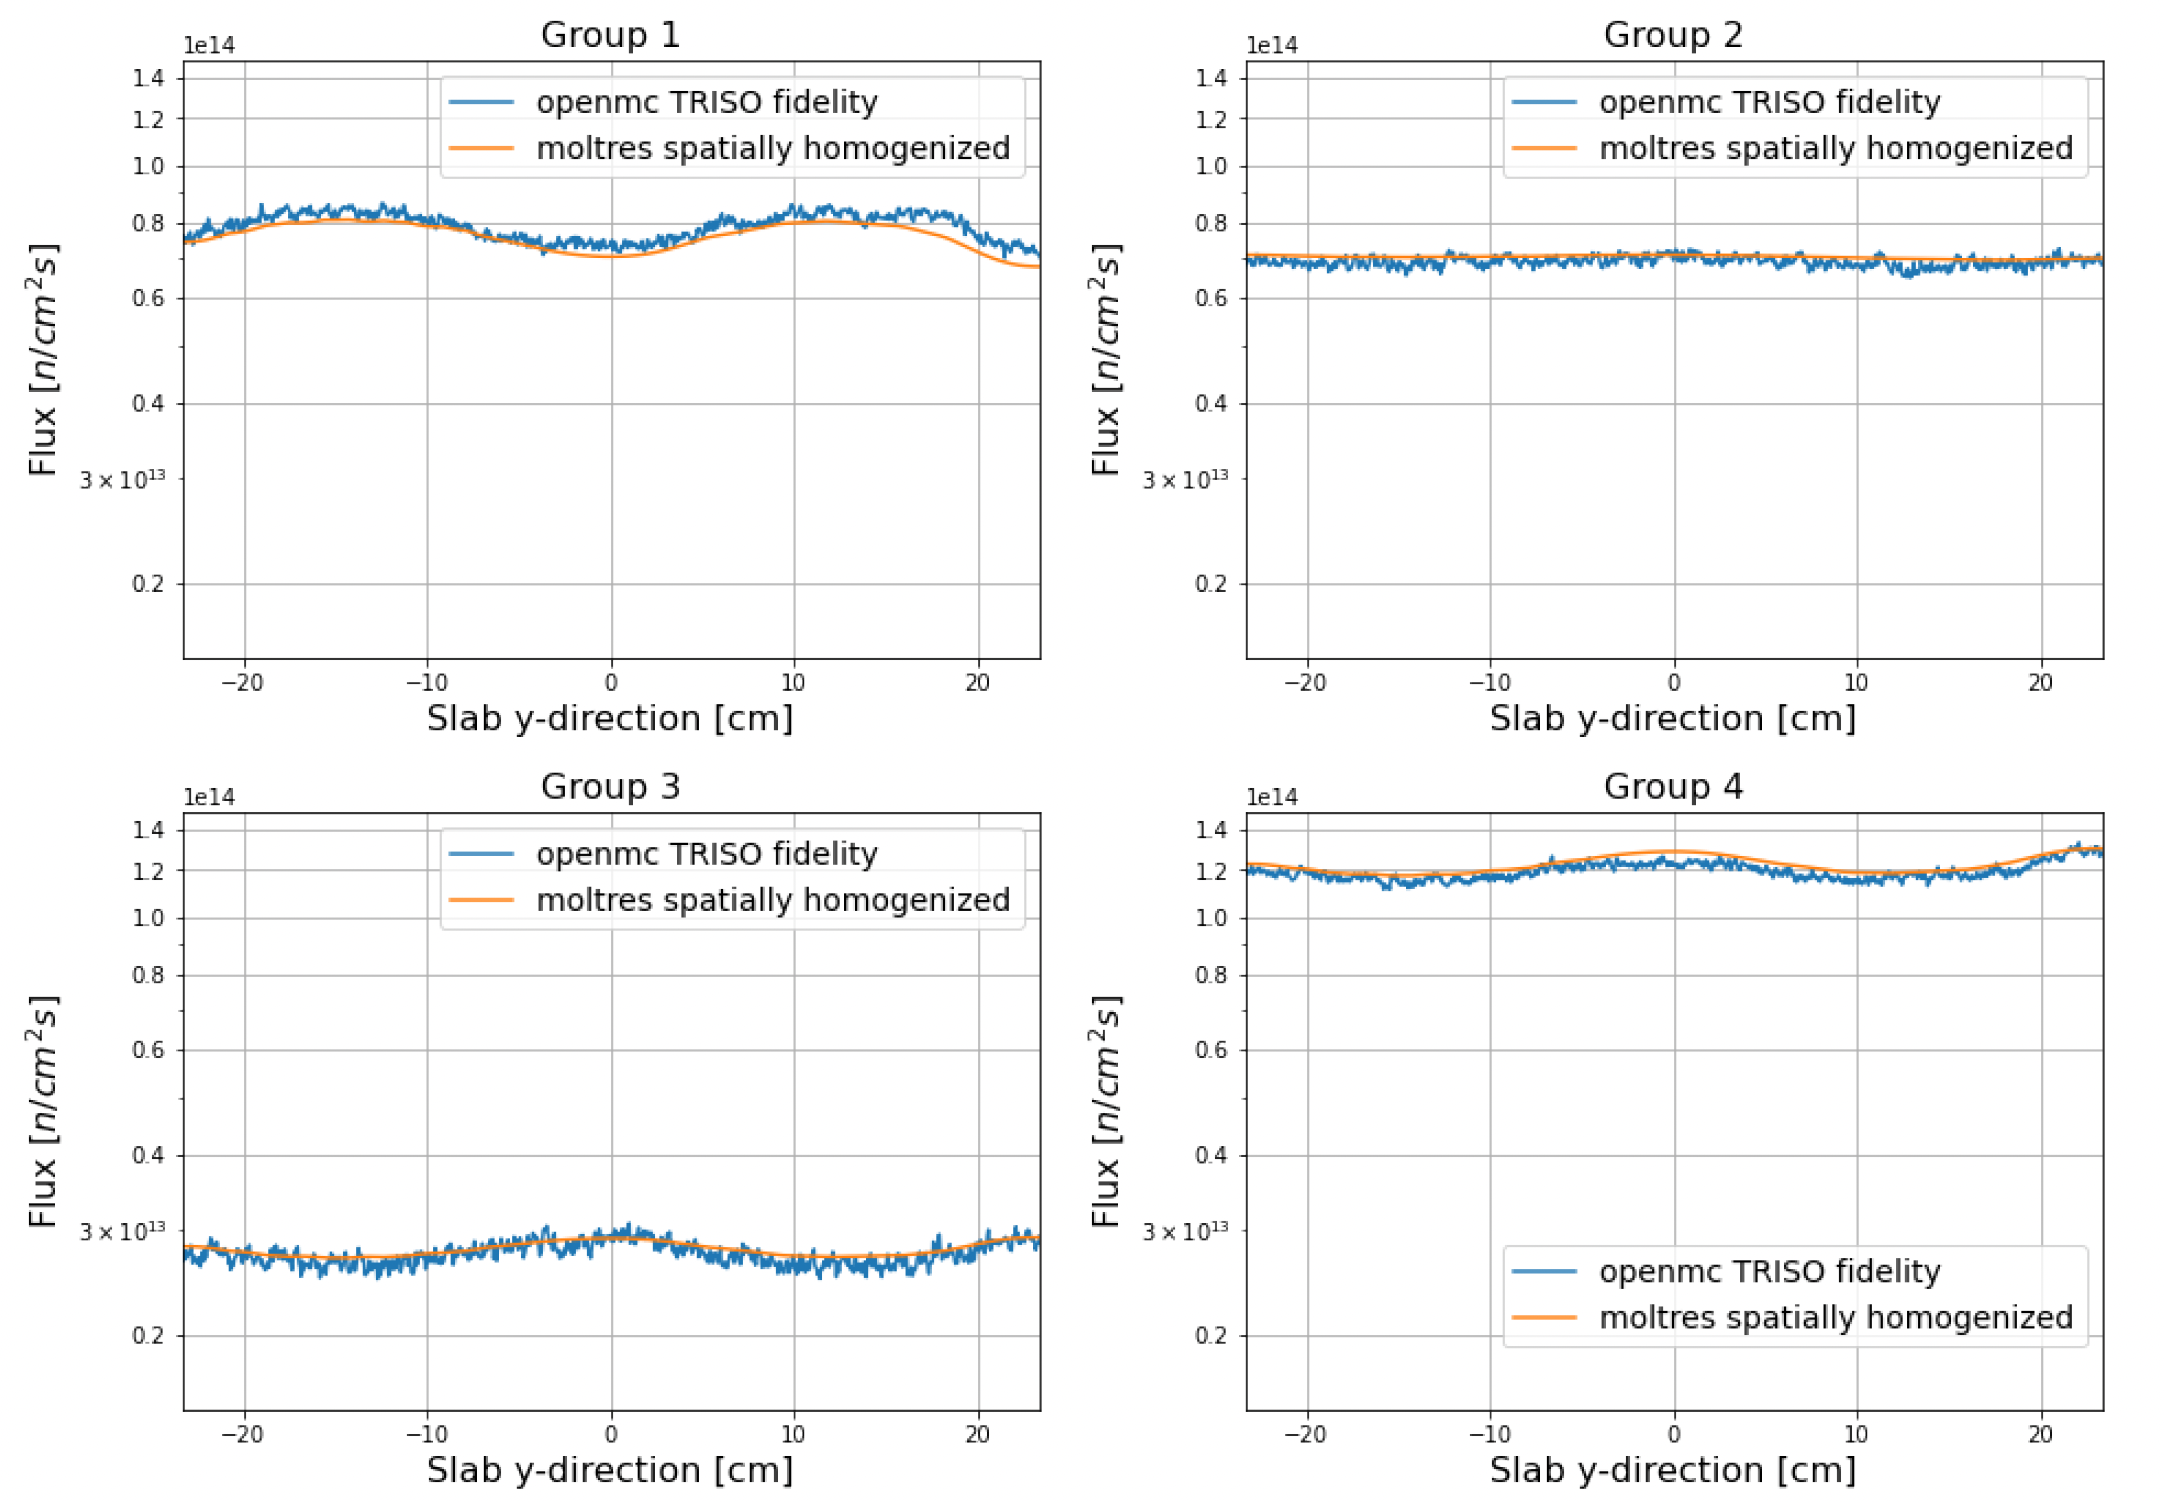
\includegraphics[width=0.8\linewidth]{figures/benchmark-flux.png} 
        \caption{4-group flux distribution comparison.}
    \end{figure}
\end{frame}

\begin{frame}
    \frametitle{AHTR Temp Model Neutron Spectrum Verification}
            \begin{figure}[]
                \centering
                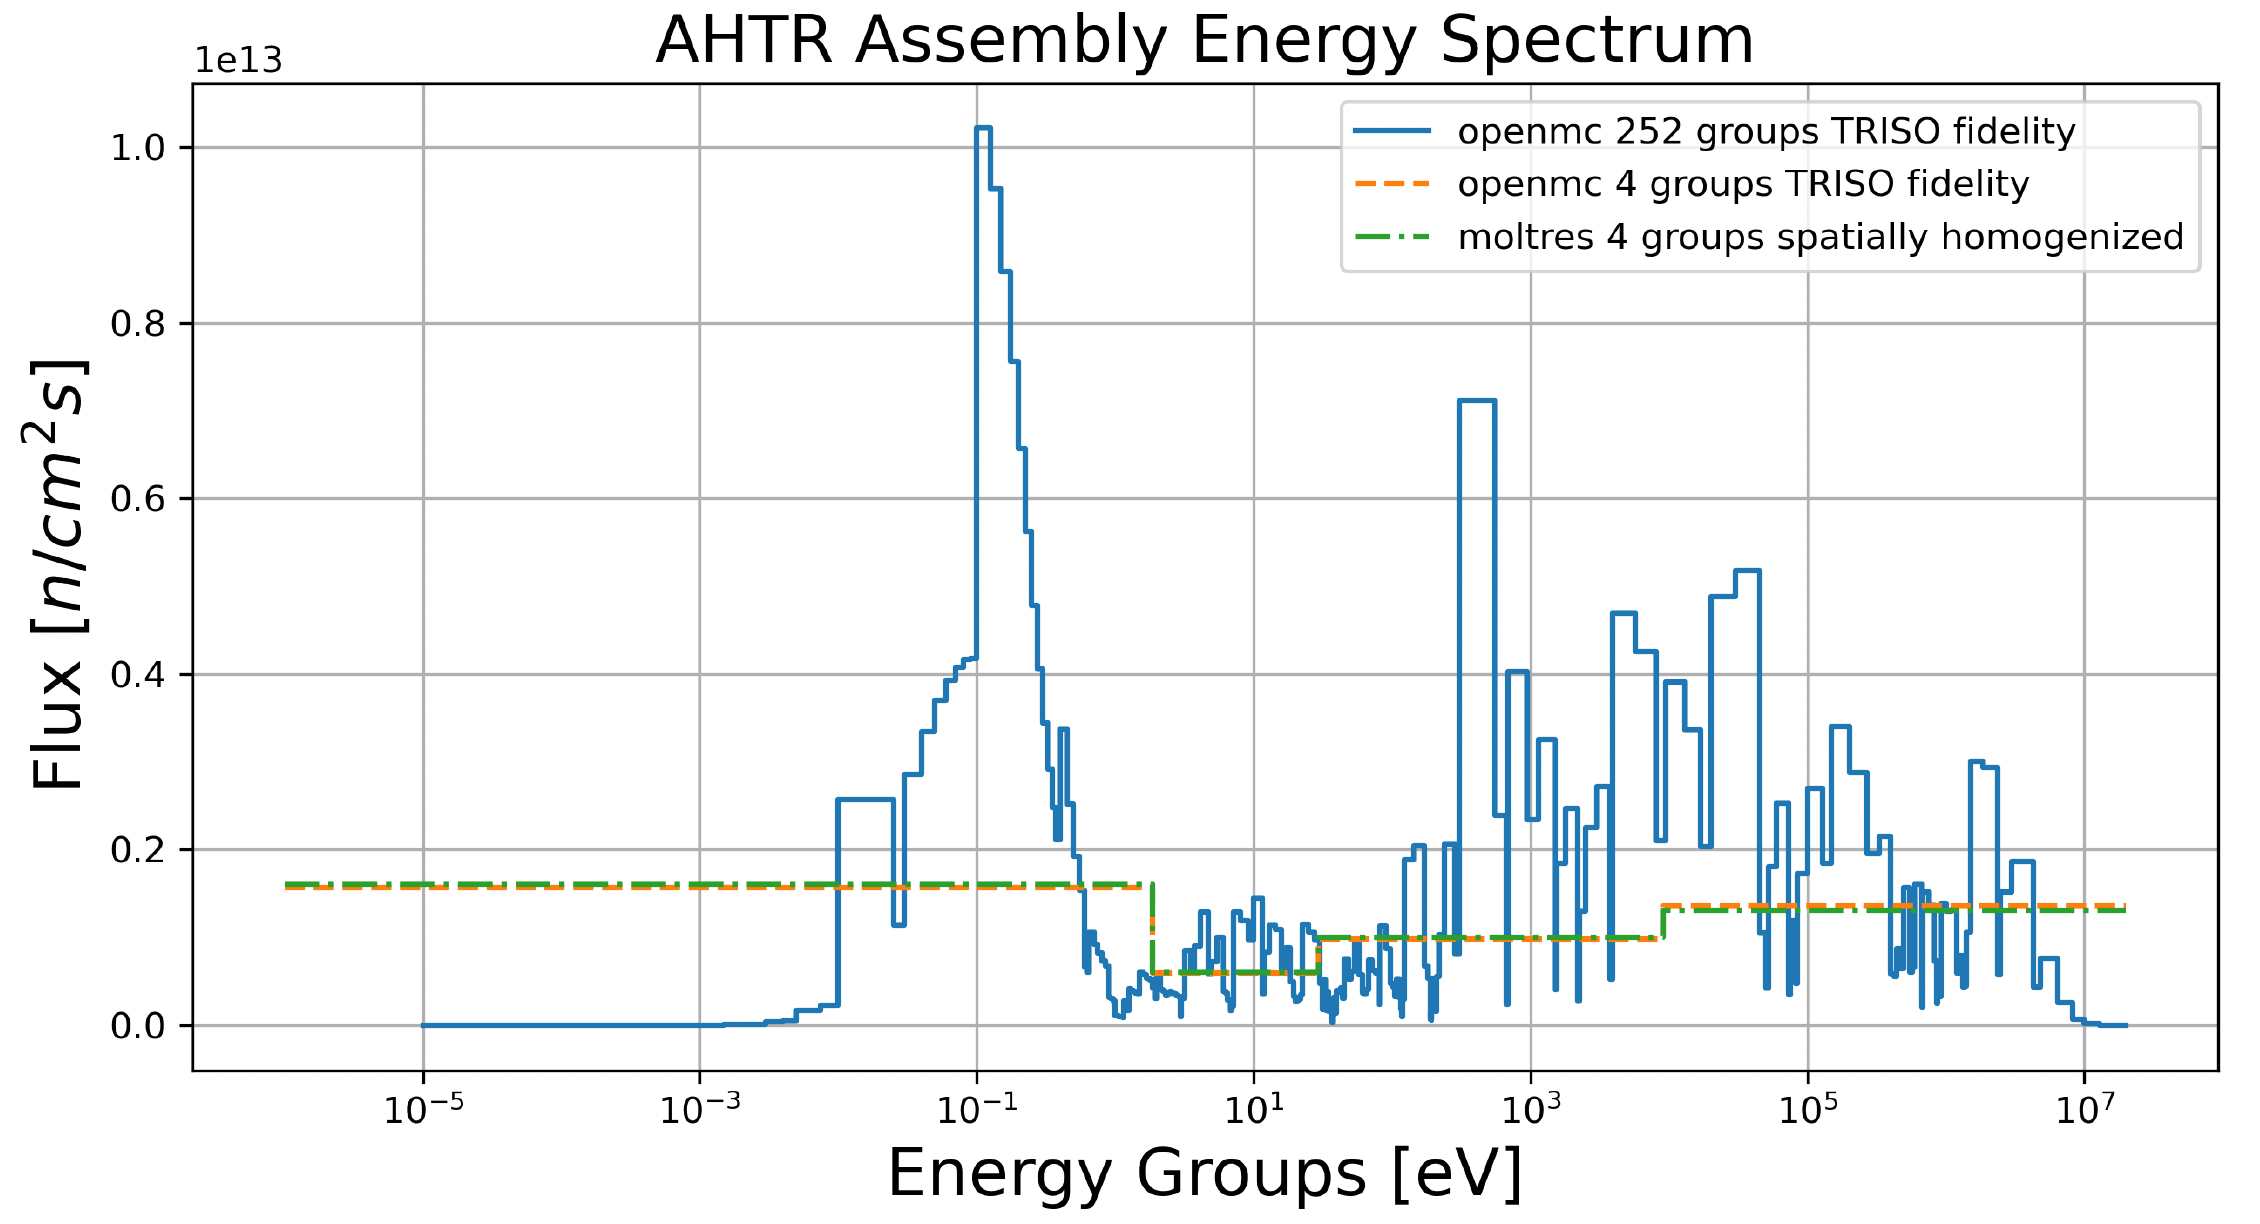
\includegraphics[width=0.75\linewidth]{figures/benchmark-spectrum.png} 
                \caption{Neutron Energy Spectrum Comparison.}
            \end{figure}
        Moltres replicated the relevant neutronics parameters with sufficient accuracy
        using OpenMC's group constant data for the AHTR full assembly model.
\end{frame}
